\documentclass[a4paper, 11pt]{article}
\usepackage{comment} % enables the use of multi-line comments (\ifx \fi) 
\usepackage{fullpage} % changes the margin
\usepackage{graphicx}
\usepackage{fancyvrb,xcolor}
\usepackage{listings}
\usepackage{color}

\definecolor{dkgreen}{rgb}{0,0.6,0}
\definecolor{gray}{rgb}{0.5,0.5,0.5}
\definecolor{mauve}{rgb}{0.58,0,0.82}

\usepackage{caption}
\DeclareCaptionFont{white}{\color{white}}
\DeclareCaptionFormat{listing}{\colorbox{gray}{\parbox{\textwidth}{#1#2#3}}}
\captionsetup[lstlisting]{format=listing,labelfont=white,textfont=white}

\lstset{
numbers=left,
backgroundcolor=\color{white},
frame=single,
tabsize=2,
captionpos=b,
breaklines=true,
breakautoindent=true,
escapeinside={\%*}{*)}
}
\graphicspath{ {images/} }

\begin{document}
%Header-Make sure you update this information!!!!
\noindent
\large\textbf{Assignment-1} \hfill \textbf{Chandrasekhar Reddy Muthyala} \\
\normalsize CS532, Web Science, Spring 2018\hfill CS Master's Student \\
Old Dominion University, Computer Science Dept \hfill Prof:  Alexander C. Nwala

\section*{Question 1:}
 Demonstrate that you know how to use "curl" well enough to correctly POST data to a form.  Show that the HTML response that is returned is "correct".  That is, the server should take the arguments you POSTed and build a response accordingly.  Save the HTML response to a file and then view that file in a browser and take a screen shot.



\subsection*{Answer:}
Data can be posted into the form by using CURL at the command line like below
curl --data  "param1=value1\&param2=value2" -X POST <URL>
--data <data> Send specified data in POST request 
-X, --request The request method to use[1].

Example: 

Let's print HTML  page using ``curl''. This page `` problem1.html'' is created for test purpose. It makes it possible to post data using a web browser:

\begin{lstlisting}[language=bash,label=Command:,caption=Command:]
curl --data  "fname=chandu\&lname=muthyala"http://qav2.cs.odu.edu/chandu/WebSciences/A1/problem1.php -o problem1.html
\end{lstlisting}
\begin{lstlisting}[language=html,label=Output:,caption=Output: The content of problem1.html]
<!DOCTYPE html>
<html>
<body>
<?php
     echo "<br>";
     echo "<br>";
     echo "<b>fname Posted: </b>" . $_POST['fname'] . "<br>";
     echo "<b>lname Posted: </b>" . $_POST['lname'] . "<br>";
?>

</body>
</html>
\end{lstlisting}
 I created a problem1.php file which contain a HTML code and expects  two parameters  fname  and lname  and these two parameters  are included inside html code to show they are posted correctly. 

\begin{lstlisting}[language=html,label=Output:,caption=Output: The output of problem1.php]     
<!DOCTYPE html>
<html>
<body>
<br /><br /><b>fname Posted: </b>chandu<br /><b>lname Posted: </b>muthyala<br />
</body>
</html>
\end{lstlisting}
We can clearly see that the response is saved to a file named ``problem1.html''.


\begin{figure}[h]
\caption{Screenshot of The file problem1.html opened in a web browser}
\centering
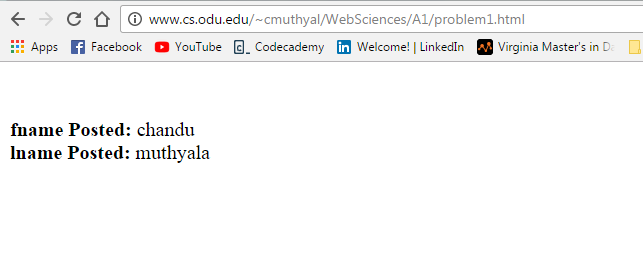
\includegraphics[scale=0.76]{problem1.png}
\end{figure}
\section*{Question 2:}
Write a Python program that:
\newline
\indent
1. Takes as a command line argument a web page
\newline
\indent
2. Extracts all the links from the page
\newline
\indent
3. Lists all the links that result in PDF files, and prints out the bytes for each of the links. 
\newline
\indent
(note: be sure to follow all the redirects until the link terminates with a ``200 OK''.)
\newline
\indent
4. show that the program works on 3 different URIs, one of which needs to be:
\newline
\indent
http://www.cs.odu.edu/\textasciitilde mln/teaching/cs532-s17/test/pdfs.html
     
\subsection*{Answer:} 
\begin{lstlisting}[language=python,label=Python-code,caption=The content of Assignment1.py]
#!/usr/bin/env python3
import sys
import requests
from bs4 import BeautifulSoup
import urllib.request
from urllib.error import  URLError
from urllib.parse import urlparse
class Assignment1:
	def __init__(self):
		self.title = "*** Extracting all the Links from a web-page. ***"
		self.vistitedLinks= []
		self.pdfList = {}
		self.movedLinks = []
		self.linkList = []

	def printSysArguments(self):
		length = len(sys.argv)
		if length>1:
			self.siteUrl = sys.argv[1]
			print("Entered URL: ",self.siteUrl)
	def returnPdfs(self, url):
		try:
			responsed = requests.get(url)
			if(responsed.history):
				res = urllib.request.urlopen(responsed.url)
				print("Final URL:",responsed.url)
			else:
				res = urllib.request.urlopen(url)
				print("Final URL:",url)

			intialStatus = responsed.status_code
			if(intialStatus==200):
				info = res.info()
				redditHtml = res.read()
				soup = BeautifulSoup(redditHtml, "html.parser")
				for link in soup.find_all('a'):
					if not link.get('href')==None:
						if not link.get('href').startswith("#") and not link.get('href')=="" and not link.get('href').startswith("?") :
							if not bool(urlparse(link.get('href')).netloc):
								finalUrl = url+link.get('href')
								linkreq = urllib.request.Request(url+link.get('href'))
							else:
								finalUrl = link.get('href')
								linkreq = urllib.request.Request(link.get('href'))
							try:
								linkRes = urllib.request.urlopen(linkreq)
								linkStatus = linkRes.getcode()
								linkContentType = linkRes.info().get_content_type()
								if linkStatus==200:
									if linkContentType == "application/pdf":
										self.linkList.append(finalUrl)
										self.pdfList[link.get('href')]=linkRes.headers['content-length']
									elif linkContentType == "text/html":
										self.linkList.append(finalUrl)
										if  link.get('href') not in self.vistitedLinks:
											self.vistitedLinks.append(link.get('href'))
								elif linkStatus>=300 and linkStatus<400:
									if link.get('href') not in self.vistitedLinks and linkRes.geturl() not in movedLinks:
										self.vistitedLinks.append(link.get('href'))
										self.vistitedLinks.append(linkRes.geturl())
										self.movedLinks.append(linkRes.geturl())
										self.returnPdfs(linkRes.geturl())
							except URLError as e:
							    if hasattr(e, 'reason'):
							    	# print('Reason: ', e.reason)
							    	pass
							    elif hasattr(e, 'code'):
							    	# print('Error code: ', e.code)
							    	pass		    	
		except URLError as e:
		    if hasattr(e, 'reason'):
		    	# print('Reason: ', e.reason)
		    	pass
		    elif hasattr(e, 'code'):
		    	# print('Error code: ', e.code)
		    	pass
					
		return self.pdfList

obj = Assignment1()
if(len(sys.argv)==2):
	obj.printSysArguments()
	listOfLinks = obj.returnPdfs(obj.siteUrl)
	if(len(listOfLinks)>0):
		print("Pdfs in the link:")
		for link in listOfLinks:
			print("\t",link,":",listOfLinks[link]," Bytes")
		for link in obj.movedLinks:
			print("moved:", link)
	else:
		print("Pdfs in the link: None")

	print("All the links in the given link:")
	for link in obj.linkList:
		print("\t",link)

else:
	print("Please provide URL along with file name.")
\end{lstlisting}
\subsection*{Running the program:}
The main aim of the below program is to extract all the Pdfs from the given URI. This program was done using python classes. When the program runs Assignment1.py, it first check whether URI is provided in the command line, if not provided will throw an error saying ‘Please provide URI along with file name’. If the checking condition is true, the URI is passing to the member function ‘returnPdfs’ of Assignment1 class. 
In the ‘returnPdfs’ function  initially checking passed URI has redirections by using ‘requests’ library and  getting the final URI  of the  passed URI . Making a first request using ‘urllib’ library in the try block, I have include an error reporting library to avoid exceptions which causes from http connection and urls.. By using ‘urllib.request’ library I am extracting the all the HTML content of the URI and passing to beautiful soap to get all the links. 
Checking whether link is absolute or not by using ‘urlparse’ library, based on that I am finding the final URL and  request is made for link in a try block to avoid http connection errors and URL errors. Getting the info of each link and extracting the header information, checking the status  code of the link If the link is with status code 200and then checking the  content-type is application/pdf  and  I am storing the link and its file size in to a dictionary. If content type is text/html I am moving that link into a visited list so that I can avoid duplicate links in displaying all the links in provided URI. In case if status code is in the range of 300-399 the URI is passed to the ‘returnPdfs’ function and process repeated as stated above. 

\noindent
\textbf{First Test Case:}
Let's test the link: 
\newline
 http://www.gmail.com
\newline
The link above is redirected to the link:
\newline
https://accounts.google.com/ServiceLogin?service=mail\&passive=true\&rm=false\&continue=https://mail.google.com/mail/\&ss=1\&scc=1\&ltmpl=default\&ltmplcache=2\&emr=1\&osid=1
\newline
\noindent
Pdfs in the links: None
\begin{lstlisting}[language=bash,label=Command:,caption=Command:]
python Assignment1.py  "http://www.gmail.com" 
\end{lstlisting}
\begin{lstlisting}[language=bash,label=Output,caption=Output:]
Entered URL:
 http://www.gmail.com
Final URL:
https://accounts.google.com/ServiceLogin?service=mail\&passive=true\&rm=false\&continue=https://mail.google.com/mail/\&ss=1\&scc=1\&ltmpl=default\&ltmplcache=2\&emr=1\&osid=1
Pdfs in the link: None
All the links in the given link:
	 https://accounts.google.com/signin/usernamerecovery?continue=https\%3A\%2F\%2Fmail.google.com\%2Fmail\%2F\&service=mail\&ss=1\&scc=1\&rm=false\&osid=1\&hl=en
	 https://accounts.google.com/AccountChooser?continue=https\%3A\%2F\%2Fmail.google.com\%2Fmail\%2F\&service=mail\&rm=false\&ltmpl=default\&scc=1\&ss=1\&osid=1\&emr=1
	 https://accounts.google.com/SignUp?service=mail\&continue=https\%3A\%2F\%2Fmail.google.com\%2Fmail\%2F\&ltmpl=default
	 https://www.google.com/intl/en/about
	 https://accounts.google.com/TOS?loc=US\&hl=en\&privacy=true
	 https://accounts.google.com/TOS?loc=US\&hl=en
	 http://www.google.com/support/accounts?hl=en
\end{lstlisting}
\noindent
\textbf{Required Test Case:}
http://www.cs.odu.edu/\textasciitilde mln/teaching/cs532-s17/test/pdfs.html
\begin{lstlisting}[language=bash,label=Command:,caption=Command:]
python Assignment1.py " http://www.cs.odu.edu/~mln/teaching/cs532-s17/test/pdfs.html"
\end{lstlisting}
\begin{lstlisting}[language=bash,label=Output:,caption=Output:]
Entered URL:  http://www.cs.odu.edu/~mln/teaching/cs532-s17/test/pdfs.html
Final URL: http://www.cs.odu.edu/~mln/teaching/cs532-s17/test/pdfs.html
Pdfs in the link:
	 http://www.cs.odu.edu/~mln/pubs/ht-2015/hypertext-2015-temporal-violations.pdf : 2184076  Bytes
	 http://www.cs.odu.edu/~mln/pubs/tpdl-2015/tpdl-2015-annotations.pdf : 622981  Bytes
	 http://arxiv.org/pdf/1512.06195 : 1748961  Bytes
	 http://www.cs.odu.edu/~mln/pubs/tpdl-2015/tpdl-2015-off-topic.pdf : 4308768  Bytes
	 http://www.cs.odu.edu/~mln/pubs/tpdl-2015/tpdl-2015-stories.pdf : 1274604  Bytes
	 http://www.cs.odu.edu/~mln/pubs/tpdl-2015/tpdl-2015-profiling.pdf : 639001  Bytes
	 http://www.cs.odu.edu/~mln/pubs/jcdl-2014/jcdl-2014-brunelle-damage.pdf : 2205546  Bytes
	 http://bit.ly/1ZDatNK : 720476  Bytes
	 http://www.cs.odu.edu/~mln/pubs/jcdl-2015/jcdl-2015-mink.pdf : 1254605  Bytes
	 http://www.cs.odu.edu/~mln/pubs/jcdl-2015/jcdl-2015-arabic-sites.pdf : 709420  Bytes
	 http://www.cs.odu.edu/~mln/pubs/jcdl-2015/jcdl-2015-dictionary.pdf : 2350603  Bytes
All the links in the given link:
	 http://twitter.com/webscidl
	 http://www.dlib.org/dlib/november15/vandesompel/11vandesompel.html
	 http://arxiv.org/abs/1508.02315
	 http://arxiv.org/abs/1508.02315
	 http://www.cs.odu.edu/~mln/pubs/ht-2015/hypertext-2015-temporal-violations.pdf
	 http://www.cs.odu.edu/~mln/pubs/tpdl-2015/tpdl-2015-annotations.pdf
	 http://arxiv.org/pdf/1512.06195
	 http://www.cs.odu.edu/~mln/pubs/tpdl-2015/tpdl-2015-off-topic.pdf
	 http://www.cs.odu.edu/~mln/pubs/tpdl-2015/tpdl-2015-stories.pdf
	 http://www.cs.odu.edu/~mln/pubs/tpdl-2015/tpdl-2015-profiling.pdf
	 http://dx.doi.org/10.1007/s00799-015-0150-6
	 http://www.cs.odu.edu/~mln/pubs/jcdl-2014/jcdl-2014-brunelle-damage.pdf
	 http://arxiv.org/abs/1506.06279
	 http://dx.doi.org/10.1007/s00799-015-0155-1
	 http://bit.ly/1ZDatNK
	 http://www.cs.odu.edu/~mln/pubs/jcdl-2015/jcdl-2015-mink.pdf
	 http://www.cs.odu.edu/~mln/pubs/jcdl-2015/jcdl-2015-arabic-sites.pdf
	 http://www.cs.odu.edu/~mln/pubs/jcdl-2015/jcdl-2015-dictionary.pdf
	 http://bit.ly/jcdl-pdf
	 http://dx.doi.org/10.1007/s00799-015-0140-8

-------------------------------------
\end{lstlisting}
\noindent
\textbf{Additional Test Case:}
 http://www.cs.odu.edu/~mweigle/
\begin{lstlisting}[language=bash,label=Command:,caption=Command:]
python Assignment1.py  " http://www.cs.odu.edu/~mweigle/" 
\end{lstlisting}
\begin{lstlisting}[language=bash,label=Output:,caption=Output:]
Entered URL:  http://www.cs.odu.edu/~mweigle/
Final URL: http://www.cs.odu.edu/~mweigle/
Pdfs in the link:
	 http://www.cs.odu.edu/~mweigle/files/CV.pdf : 101583  Bytes
	 http://www.cs.odu.edu/~mweigle/papers/alkwai-tois17-preprint.pdf : 1430568  Bytes
	 http://www.cs.odu.edu/~mweigle/papers/alam-jcdl17.pdf : 1600140  Bytes
	 http://www.cs.odu.edu/~anwala/files/publications/NwalaJCDL_LMP.pdf : 17623699  Bytes
	 http://www.cs.odu.edu/~mweigle/papers/alnoamany-websci17.pdf : 6962016  Bytes
	 http://www.cs.odu.edu/~mweigle/papers/brunelle-jcdl17.pdf : 1276346  Bytes
	 http://www.cs.odu.edu/~mkelly/papers/2017_jcdl_wail.pdf : 412476  Bytes
	 http://www.cs.odu.edu/~mkelly/papers/2017_jcdl_countingMementos.pdf : 274265  Bytes
	 http://www.cs.odu.edu/~mln/pubs/jcdl-2015/jcdl-2015-mink.pdf : 1254605  Bytes
	 http://www.cs.odu.edu/~mln/pubs/jcdl-2015/jcdl-2015-arabic-sites.pdf : 709420  Bytes
	 http://www.cs.odu.edu/~mweigle/papers/mohrehkesh-misenet14.pdf : 1231147  Bytes
	 http://www.cs.odu.edu/~mln/pubs/jcdl-2014/jcdl-2014-brunelle-damage.pdf : 2205546  Bytes
	 http://www.cs.odu.edu/~mweigle/papers/olariu-misenet13.pdf : 405542  Bytes
	 http://www.cs.odu.edu/~mln/pubs/tpdl-2013/paper_149.pdf : 813692  Bytes
	 http://www.cs.odu.edu/~mweigle/papers/yan-soli09.pdf : 278184  Bytes
All the links in the given link:
	 http://www.cs.odu.edu
	 http://www.odu.edu
	 http://www.cs.odu.edu/~mweigle/Main/Home?action=login
	 http://www.cs.odu.edu/~mweigle/Main/Home
	 http://www.cs.odu.edu/~mweigle/Main/Research
	 http://www.cs.odu.edu/~mweigle/Main/PubsByYear
	 http://www.cs.odu.edu/~mweigle/Main/Students
	 http://www.cs.odu.edu/~mweigle/files/CV.pdf
	 http://www.cs.odu.edu/~mweigle/Resources/WorkingWithMe
	 http://www.cs.odu.edu/~mweigle/Resources/ResearchMethods
	 http://www.cs.odu.edu/~mweigle/Resources/InfoVis
	 http://www.cs.odu.edu/~mweigle/Main/Teaching
	 http://www.cs.odu.edu/~mweigle/Main/Sched
	 http://www.cs.odu.edu/~mweigle/Main/Personal
	 http://www.cs.odu.edu/~mweigle/CS725-S18/Home
	 https://graduate.cs.odu.edu/
	 http://www.cs.odu.edu/~yaohang
	 https://securegrants.neh.gov/publicquery/main.aspx?f=1&gn=HAA-256368-17
	 https://www.neh.gov/divisions/odh/grant-news/announcing-new-2017-odh-grant-awards
	 http://ws-dl.blogspot.com
	 http://ws-dl.blogspot.com/2018/01/2018-01-08-introducing-reconstructive.html
	 http://ws-dl.blogspot.com/2018/01/2018-01-07-review-of-ws-dls-2017.html
	 http://ws-dl.blogspot.com/2018/01/2018-01-06-two-wsdl-classes-offered-for.html
	 http://ws-dl.blogspot.com/2018/01/2018-01-02-link-to-web-archives-not.html
	 http://ws-dl.blogspot.com/2017/12/2017-12-31-digital-blackness-in-archive.html
	 http://www.cs.odu.edu/~mweigle/Research/InfoVis-Gallery
	 https://arxiv.org/abs/1712.03140
	 http://www.cs.odu.edu/~mweigle/Main/Home?action=bibentry&bibfile=Main.bibtex&bibref=aturban-arxiv17
	 https://arxiv.org/abs/1708.05790
	 http://www.cs.odu.edu/~mweigle/Main/Home?action=bibentry&bibfile=Main.bibtex&bibref=mccoy-arxiv17
	 http://www.cs.odu.edu/~mweigle/papers/alkwai-tois17-preprint.pdf
	 http://www.cs.odu.edu/~mweigle/Main/Home?action=bibentry&bibfile=Main.bibtex&bibref=alkwai-tois17
	 http://www.cs.odu.edu/~mweigle/papers/alam-jcdl17.pdf
	 http://www.cs.odu.edu/~mweigle/Main/Home?action=bibentry&bibfile=Main.bibtex&bibref=alam-jcdl17
	 http://www.cs.odu.edu/~anwala/files/publications/NwalaJCDL_LMP.pdf
	 http://www.cs.odu.edu/~mweigle/Main/Home?action=bibentry&bibfile=Main.bibtex&bibref=nwala-jcdl17
	 http://www.cs.odu.edu/~mweigle/papers/alnoamany-websci17.pdf
	 http://www.cs.odu.edu/~mweigle/Main/Home?action=bibentry&bibfile=Main.bibtex&bibref=alnoamany-websci17
	 http://www.cs.odu.edu/~mweigle/papers/brunelle-jcdl17.pdf
	 http://www.cs.odu.edu/~mweigle/Main/Home?action=bibentry&bibfile=Main.bibtex&bibref=brunelle-jcdl17
	 http://dx.doi.org/10.1109/JCDL.2017.7991619
	 http://www.cs.odu.edu/~mkelly/papers/2017_jcdl_wail.pdf
	 http://www.cs.odu.edu/~mweigle/Main/Home?action=bibentry&bibfile=Main.bibtex&bibref=berlin-jcdl17
	 http://dx.doi.org/10.1109/JCDL.2017.7991601
	 http://www.cs.odu.edu/~mkelly/papers/2017_jcdl_countingMementos.pdf
	 http://www.cs.odu.edu/~mweigle/Main/Home?action=bibentry&bibfile=Main.bibtex&bibref=kelly-jcdl17
	 http://arxiv.org/abs/1705.06218
	 http://www.cs.odu.edu/~mweigle/Main/Home?action=bibentry&bibfile=Main.bibtex&bibref=alnoamany-arxiv17
	 http://dx.doi.org/10.1109/JCDL.2017.7991601
	 http://www.cs.odu.edu/~mkelly/papers/2017_jcdl_countingMementos.pdf
	 http://www.cs.odu.edu/~mweigle/Main/Home?action=bibentry&bibfile=Main.bibtex&bibref=kelly-jcdl17
	 http://www.cs.odu.edu/~mln/pubs/jcdl-2015/jcdl-2015-mink.pdf
	 http://www.cs.odu.edu/~mweigle/Main/Home?action=bibentry&bibfile=Main.bibtex&bibref=jordan-jcdl15
	 http://www.cs.odu.edu/~mln/pubs/jcdl-2015/jcdl-2015-arabic-sites.pdf
	 http://www.cs.odu.edu/~mweigle/Main/Home?action=bibentry&bibfile=Main.bibtex&bibref=alkwai-jcdl15
	 http://dx.doi.org/10.1109/MASS.2014.91
	 http://www.cs.odu.edu/~mweigle/papers/mohrehkesh-misenet14.pdf
	 http://www.cs.odu.edu/~mweigle/Main/Home?action=bibentry&bibfile=Main.bibtex&bibref=mohrehkesh-misenet14
	 http://dx.doi.org/10.1109/JCDL.2014.6970187
	 http://www.cs.odu.edu/~mln/pubs/jcdl-2014/jcdl-2014-brunelle-damage.pdf
	 http://www.cs.odu.edu/~mweigle/Main/Home?action=bibentry&bibfile=Main.bibtex&bibref=brunelle-jcdl14
	 http://www.cs.odu.edu/~mweigle/papers/olariu-misenet13.pdf
	 http://www.cs.odu.edu/~mweigle/Main/Home?action=bibentry&bibfile=Main.bibtex&bibref=olariu-misenet13
	 http://dx.doi.org/10.1007/978-3-642-40501-3_35
	 http://www.cs.odu.edu/~mln/pubs/tpdl-2013/paper_149.pdf
	 http://arxiv.org/abs/1309.4016
	 http://www.cs.odu.edu/~mweigle/Main/Home?action=bibentry&bibfile=Main.bibtex&bibref=alnoamany-tpdl13
	 http://dx.doi.org/10.1109/SOLI.2009.5203967
	 http://www.cs.odu.edu/~mweigle/papers/yan-soli09.pdf
	 http://www.cs.odu.edu/~mweigle/Main/Home?action=bibentry&bibfile=Main.bibtex&bibref=yan-soli09
	 https://securegrants.neh.gov/publicquery/main.aspx?f=1&gn=HAA-256368-17
	 https://mellon.org/grants/grants-database/grants/old-dominion-university/11600663/
	 http://www.nsf.gov/awardsearch/showAward?AWD_ID=1526700
	 http://www.imls.gov/grants/awarded/lg-71-15-0077-15
	 http://www.cs.odu.edu/~mweigle/files/CV.pdf
	 http://www.cs.odu.edu/~acmw
	 http://www.ncwit.org/alliances/aa
	 http://www.cs.odu.edu/
	 http://www.odu.edu/
	 http://www.clemson.edu/ces/departments/computing/
	 http://www.clemson.edu
	 http://www.cs.unc.edu
	 http://www.unc.edu
	 http://www.ulm.edu/cba/computerscience/index.html
	 http://www.ulm.edu/honors
	 http://www.ulm.edu
	 http://www.cs.odu.edu/~mweigle/Main/Home?action=print
	 http://www.cs.odu.edu/~mweigle/Site/Search
	 http://www.cs.odu.edu/~mweigle/Main/Home?action=login

-------------------------------------
\end{lstlisting}

\ifx
\newline
\noindent
\textbf{Note:}
The file README contains the following:
\begin{itemize}
\item 
How to use the program
\item 
Required Python version
\item
Required Libraries 
\end{itemize}
\fi
\section*{Question 3:}
Consider the ``bow-tie'' graph in the Broder et al. paper (fig 9):
    http://www9.org/w9cdrom/160/160.html
    Now consider the following graph:
\newline
    A $\longrightarrow$ B
    
    B $\longrightarrow$ C
    
    C $\longrightarrow$ D
    
    C $\longrightarrow$ A
    
    C $\longrightarrow$ G
    
    E $\longrightarrow$ F
    
    G $\longrightarrow$ C
    
    G $\longrightarrow$ H
    
    I $\longrightarrow$ H
    
    I $\longrightarrow$ K
    
    L $\longrightarrow$ D
    
    M $\longrightarrow$ A
    
    M $\longrightarrow$ N
    
    N $\longrightarrow$ D
    
    O $\longrightarrow$ A
    
    P $\longrightarrow$ G 
    
    For the above graph, give the values for: IN, SCC, OUT, Tendrils, Tubes, Disconnected.
\subsection*{Answer:}
IN: O, M, P
\newline
These values are considered the \emph{IN} values due to the fact that they can reach values that are considered to be in the \emph{SCC} and also because they can't be reached from the \emph{SCC}
\noindent
\newline
SCC: A, B, C G
\newline
These values are considered the \emph{SCC} values because they are at the ``heart of the graph.'' They either are all nodes that can reach another node along directed links. This can consist of links from the outside in, nodes inside the \emph{SCC} pointing to other nodes inside, or nodes point from the inside out .
\noindent
\newline
OUT: H, D
\newline
These values are part of the \emph{OUT} because they are accessible from the \emph{SCC} but they cannot link back into it .
\noindent
\newline
Tendrils: I, K, L
\newline
These values don't reference the \emph{SCC} at any point, but do have links to the \emph{OUT} nodes and therefore they are considered the \emph{tendrils}

\noindent
\newline
Tubes: N. (There is one tube that runs from M to N to D).
\newline
This value isn't part of the ``heart of the graph'' but it does connect an \emph{IN} node to an \emph{OUT} node in one step, not touching the \emph{SCC} in the process
\noindent
\newline
Disconnected: E, F
\newline
These two values are as their title describes - disconnected. They aren't part of the \emph{SCC} and don't connect to anything else on the graph.
\begin{figure}[h]
\caption{Bowtie graph}
\centering
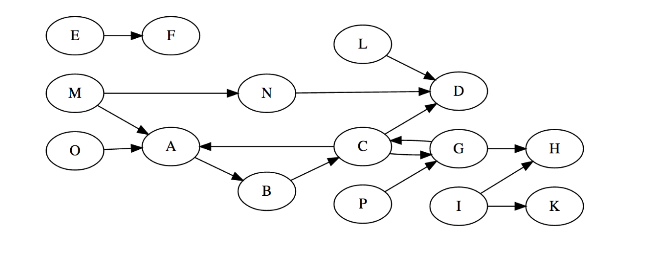
\includegraphics[scale=0.5]{bowtie.png}
\end{figure}
\subsection*{Included Files:}
bowtie.png
\begin{thebibliography}{9}
\bibitem{curl basics commands} ttps://gist.github.com/subfuzion/08c5d85437d5d4f00e58.

\end{thebibliography}
\end{document}